% Options for packages loaded elsewhere
\PassOptionsToPackage{unicode}{hyperref}
\PassOptionsToPackage{hyphens}{url}
\PassOptionsToPackage{dvipsnames,svgnames,x11names}{xcolor}
%
\documentclass[
  letterpaper,
  DIV=11,
  numbers=noendperiod]{scrartcl}

\usepackage{amsmath,amssymb}
\usepackage{lmodern}
\usepackage{iftex}
\ifPDFTeX
  \usepackage[T1]{fontenc}
  \usepackage[utf8]{inputenc}
  \usepackage{textcomp} % provide euro and other symbols
\else % if luatex or xetex
  \usepackage{unicode-math}
  \defaultfontfeatures{Scale=MatchLowercase}
  \defaultfontfeatures[\rmfamily]{Ligatures=TeX,Scale=1}
\fi
% Use upquote if available, for straight quotes in verbatim environments
\IfFileExists{upquote.sty}{\usepackage{upquote}}{}
\IfFileExists{microtype.sty}{% use microtype if available
  \usepackage[]{microtype}
  \UseMicrotypeSet[protrusion]{basicmath} % disable protrusion for tt fonts
}{}
\makeatletter
\@ifundefined{KOMAClassName}{% if non-KOMA class
  \IfFileExists{parskip.sty}{%
    \usepackage{parskip}
  }{% else
    \setlength{\parindent}{0pt}
    \setlength{\parskip}{6pt plus 2pt minus 1pt}}
}{% if KOMA class
  \KOMAoptions{parskip=half}}
\makeatother
\usepackage{xcolor}
\setlength{\emergencystretch}{3em} % prevent overfull lines
\setcounter{secnumdepth}{-\maxdimen} % remove section numbering
% Make \paragraph and \subparagraph free-standing
\ifx\paragraph\undefined\else
  \let\oldparagraph\paragraph
  \renewcommand{\paragraph}[1]{\oldparagraph{#1}\mbox{}}
\fi
\ifx\subparagraph\undefined\else
  \let\oldsubparagraph\subparagraph
  \renewcommand{\subparagraph}[1]{\oldsubparagraph{#1}\mbox{}}
\fi


\providecommand{\tightlist}{%
  \setlength{\itemsep}{0pt}\setlength{\parskip}{0pt}}\usepackage{longtable,booktabs,array}
\usepackage{calc} % for calculating minipage widths
% Correct order of tables after \paragraph or \subparagraph
\usepackage{etoolbox}
\makeatletter
\patchcmd\longtable{\par}{\if@noskipsec\mbox{}\fi\par}{}{}
\makeatother
% Allow footnotes in longtable head/foot
\IfFileExists{footnotehyper.sty}{\usepackage{footnotehyper}}{\usepackage{footnote}}
\makesavenoteenv{longtable}
\usepackage{graphicx}
\makeatletter
\def\maxwidth{\ifdim\Gin@nat@width>\linewidth\linewidth\else\Gin@nat@width\fi}
\def\maxheight{\ifdim\Gin@nat@height>\textheight\textheight\else\Gin@nat@height\fi}
\makeatother
% Scale images if necessary, so that they will not overflow the page
% margins by default, and it is still possible to overwrite the defaults
% using explicit options in \includegraphics[width, height, ...]{}
\setkeys{Gin}{width=\maxwidth,height=\maxheight,keepaspectratio}
% Set default figure placement to htbp
\makeatletter
\def\fps@figure{htbp}
\makeatother

\KOMAoption{captions}{tableheading}
\makeatletter
\makeatother
\makeatletter
\makeatother
\makeatletter
\@ifpackageloaded{caption}{}{\usepackage{caption}}
\AtBeginDocument{%
\ifdefined\contentsname
  \renewcommand*\contentsname{Table of contents}
\else
  \newcommand\contentsname{Table of contents}
\fi
\ifdefined\listfigurename
  \renewcommand*\listfigurename{List of Figures}
\else
  \newcommand\listfigurename{List of Figures}
\fi
\ifdefined\listtablename
  \renewcommand*\listtablename{List of Tables}
\else
  \newcommand\listtablename{List of Tables}
\fi
\ifdefined\figurename
  \renewcommand*\figurename{Figure}
\else
  \newcommand\figurename{Figure}
\fi
\ifdefined\tablename
  \renewcommand*\tablename{Table}
\else
  \newcommand\tablename{Table}
\fi
}
\@ifpackageloaded{float}{}{\usepackage{float}}
\floatstyle{ruled}
\@ifundefined{c@chapter}{\newfloat{codelisting}{h}{lop}}{\newfloat{codelisting}{h}{lop}[chapter]}
\floatname{codelisting}{Listing}
\newcommand*\listoflistings{\listof{codelisting}{List of Listings}}
\makeatother
\makeatletter
\@ifpackageloaded{caption}{}{\usepackage{caption}}
\@ifpackageloaded{subcaption}{}{\usepackage{subcaption}}
\makeatother
\makeatletter
\@ifpackageloaded{tcolorbox}{}{\usepackage[many]{tcolorbox}}
\makeatother
\makeatletter
\@ifundefined{shadecolor}{\definecolor{shadecolor}{rgb}{.97, .97, .97}}
\makeatother
\makeatletter
\makeatother
\ifLuaTeX
  \usepackage{selnolig}  % disable illegal ligatures
\fi
\IfFileExists{bookmark.sty}{\usepackage{bookmark}}{\usepackage{hyperref}}
\IfFileExists{xurl.sty}{\usepackage{xurl}}{} % add URL line breaks if available
\urlstyle{same} % disable monospaced font for URLs
\hypersetup{
  pdftitle={Language Models},
  pdfauthor={Kenneth Leo},
  colorlinks=true,
  linkcolor={blue},
  filecolor={Maroon},
  citecolor={Blue},
  urlcolor={Blue},
  pdfcreator={LaTeX via pandoc}}

\title{Language Models}
\author{Kenneth Leo}
\date{}

\begin{document}
\maketitle
\ifdefined\Shaded\renewenvironment{Shaded}{\begin{tcolorbox}[enhanced, sharp corners, borderline west={3pt}{0pt}{shadecolor}, frame hidden, breakable, interior hidden, boxrule=0pt]}{\end{tcolorbox}}\fi

Language models are an important part of natural language processing
(NLP) since they provide a way for computers to process or understand
the natural language and to be able to extract information that can be
used in different applications. These \textbf{natural language} are
something that is being used by humans and evolves naturally through
repetitive use (speech, sign language, non-verbal cues).

\hypertarget{what-is-a-language-model}{%
\subsection{What is a language model?}\label{what-is-a-language-model}}

In its simplest form, a language model is a probability distribution
such that, given a sequence of words, a language model will give the
probability of all the words being chosen next in the available
vocabulary. For example, given a series of words
\(w_{1:(t-1)} = (w_1,...,w_{t-1})\), a language model will give us the
probability of all words in its vocabulary \(V\) to appear next to the
series of words. \[
P(w_t | w_{1:(t-1)}), \ \ \ \ \ \ \ w_1,...,w_{t-1}\in V
\]

So if we want our model to complete our sentence, we select the word
which has the highest probability and then put that word to the series
of words and then use the model again to generate the next word. So the
essence of a language model is to simply imitate how a human would
respond to different prompts.

To give an idea of what a language model can do, let us look at the
ChatGPT, see Figure~\ref{fig-gpt}, which is an artificial intelligence
(AI) chatbot that is developed by OpenAI last November 2022.

\begin{figure}

{\centering \includegraphics{Figures_LLM/chat_gpt_sample.gif}

}

\caption{\label{fig-gpt}Example of a language model (ChatGPT)}

\end{figure}

We asked the AI to explain quantum computing in simple terms and we see
how it was able to provide an extensive discsussion of what quantum
computing is. Now, the reason why these AI chatbots are gaining such
traction is that it serves as a good starting point when writing or when
you want to gain a better understanding of topics that were not
discussed properly for example.

\hypertarget{neural-network-based-language-model-types-of-language-models}{%
\subsection{Neural Network-Based Language Model (Types of Language
Models)}\label{neural-network-based-language-model-types-of-language-models}}

ChatGPT is an example of a generative pre-trained transformer (GPT)
which is a type of language model that relies on deep learning that
generates texts based on a given input text.

\hypertarget{evolution-of-language-models}{%
\subsection{Evolution of Language
Models}\label{evolution-of-language-models}}

\hypertarget{training-language-models}{%
\subsection{Training Language Models}\label{training-language-models}}

Focusing on the transformer models, we need to know how the neural
network model is being trained: including the \emph{pre-training} and
\emph{fine-tuning} processes. In pre-training process, we provide a
general language model that has a good understarding of how language is
being used in a variety of settings.

For a neural network, we use \(n\) inputs and then it is processed in
several hidden layers until it reaches an output layer. Ideally, we want
the output of our neural network to be close to the actual/real output.
If that is not the case, then we use \textbf{gradient descent} to change
the parameters to reduce the loss function of our network. In gradient
descent, what happens is we use the output and compute some values and
then feed it back to our hidden layers until the loss is minimized,
which is why the process is also called backpropagation, see
Figure~\ref{fig-neural}.

\begin{figure}

{\centering 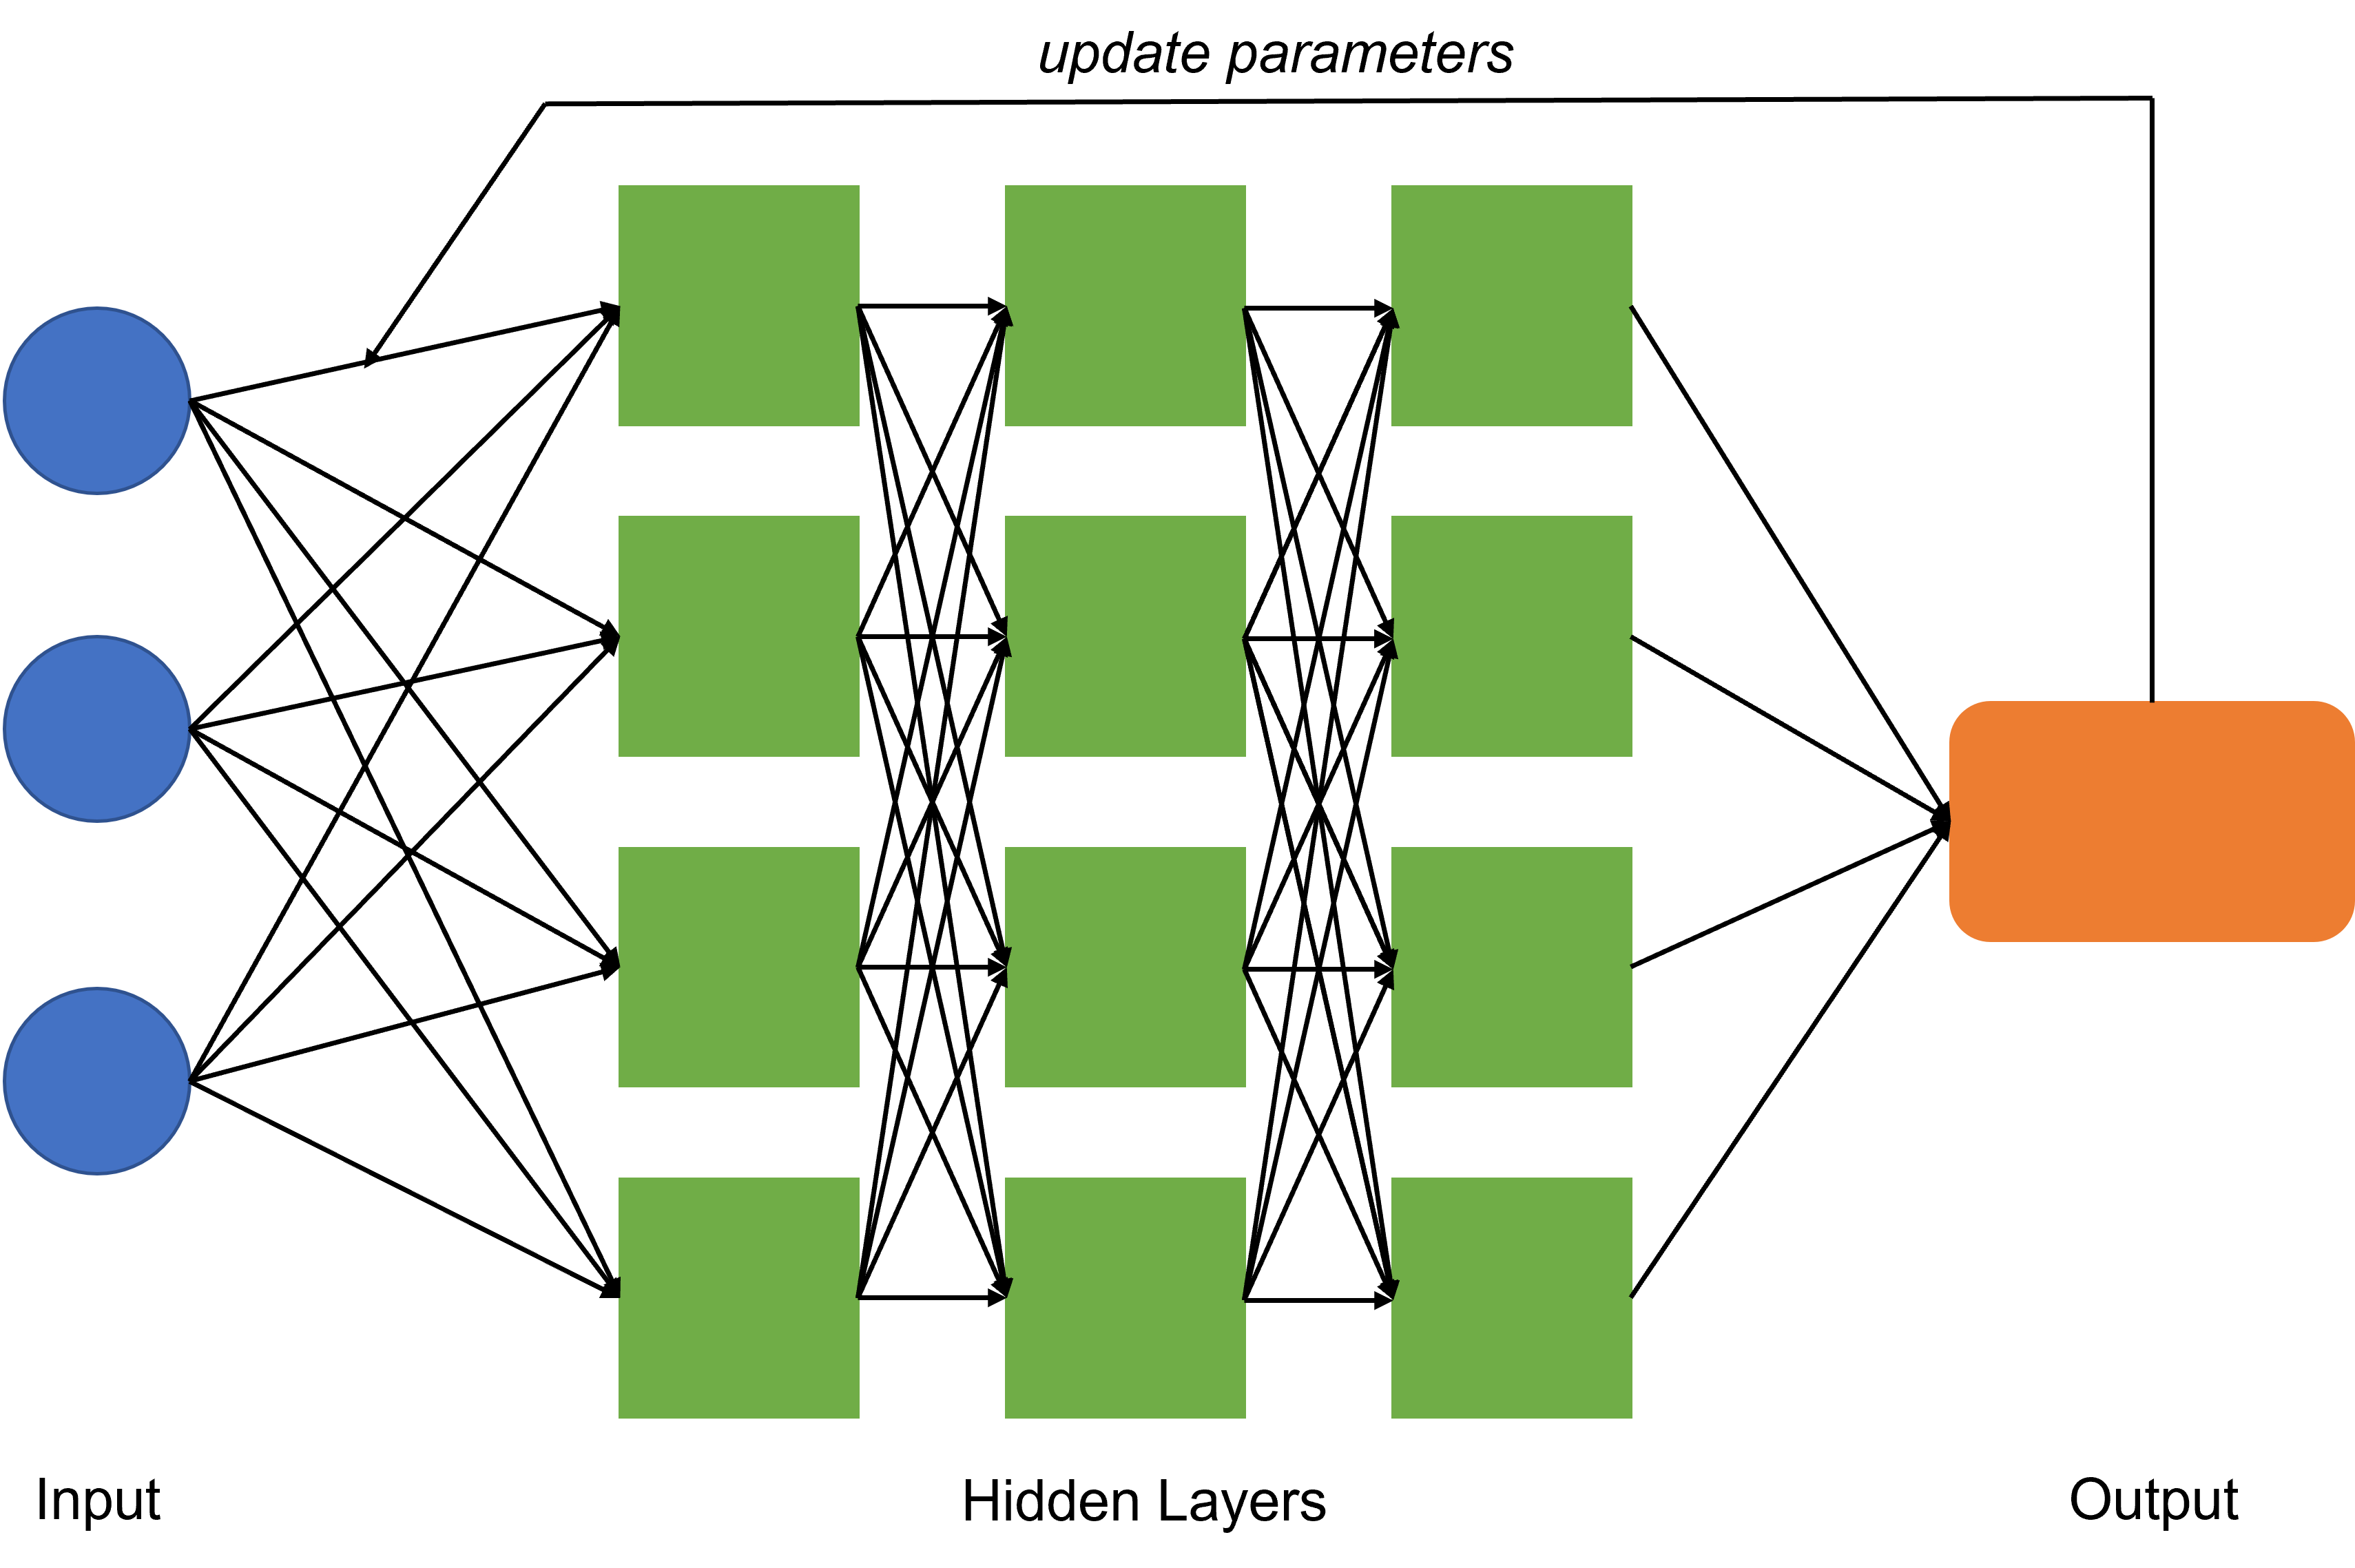
\includegraphics{Figures_LLM/neural_network.png}

}

\caption{\label{fig-neural}Simplified Neural Network}

\end{figure}

One problem of the neural network above is that the input size is fixed
and in general, we would want to process input sizes that are longer or
shorter. Now in the field of language moelling, there are two types of
networks that were considered state of the art: \emph{recurrent neural
networks} and \emph{long short-term memory networks}.

\hypertarget{recurrent-neural-networks-rnns}{%
\paragraph{Recurrent neural networks
(RNNs)}\label{recurrent-neural-networks-rnns}}

In a recurrent neural network, we still have the same neural network
discussed above to every word in a series of words. Whats different for
RNNs is that last word (newest word) in the sequence of words has the
most influence in choosing the next word and the probability of
influence of previous words reduce exponentially as new words are being
introduced. We see in Figure~\ref{fig-rnn} how RNNs are able to connect
information (or words) in a sequential manner.

\begin{figure}

{\centering 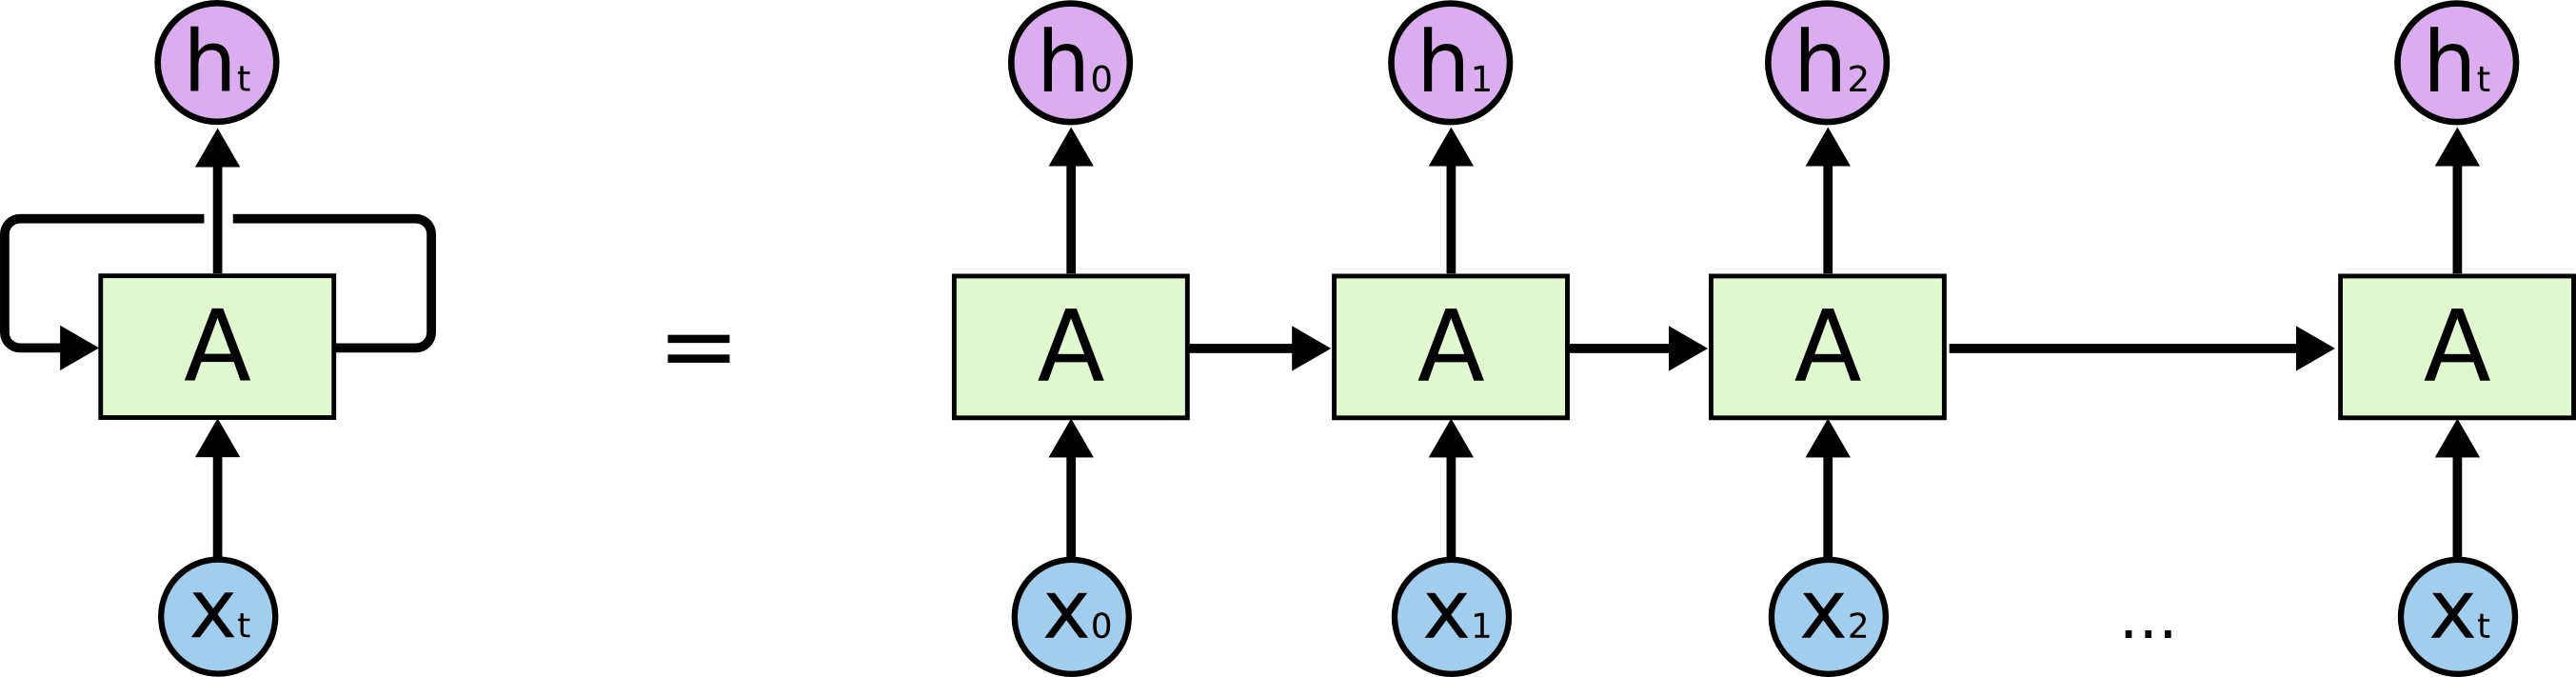
\includegraphics{Figures_LLM/rnn.png}

}

\caption{\label{fig-rnn}Recurring Neural Network}

\end{figure}

This makes sense but the problem is, language in itself is more nuanced
in the sense that sometimes we need to take into account not only the
last word in our sentence but the sentence as a whole. For example, in
Figure~\ref{fig-rnn}, if we need the output \(h_{10}\), the information
from the input \(x_1\) has very little effect on the output and this
might pose a problem if we are for example dealing with a sentence whose
subject and verb are very far from each other. Because of this unique
feature of language, the concept of older worlds having less influence
becomes a bug and is called the \emph{vanishing gradients} problem

\hypertarget{long-short-term-memory-lstm-networks}{%
\paragraph{Long short-term memory (LSTM)
networks}\label{long-short-term-memory-lstm-networks}}

Now LSTMs solve the \emph{vanishing gradients} problem by introducing a
``memory'' state whose influence is determined by gates defined by more
learnable parameters. The main difference of LSTM fromm RNN is that the
former type of network remembers information for long periods of time by
default but has there functions, called gates that can either use the
information stored to process the output or to ``forget'' the previous
information and not use for the output.

\begin{figure}

{\centering 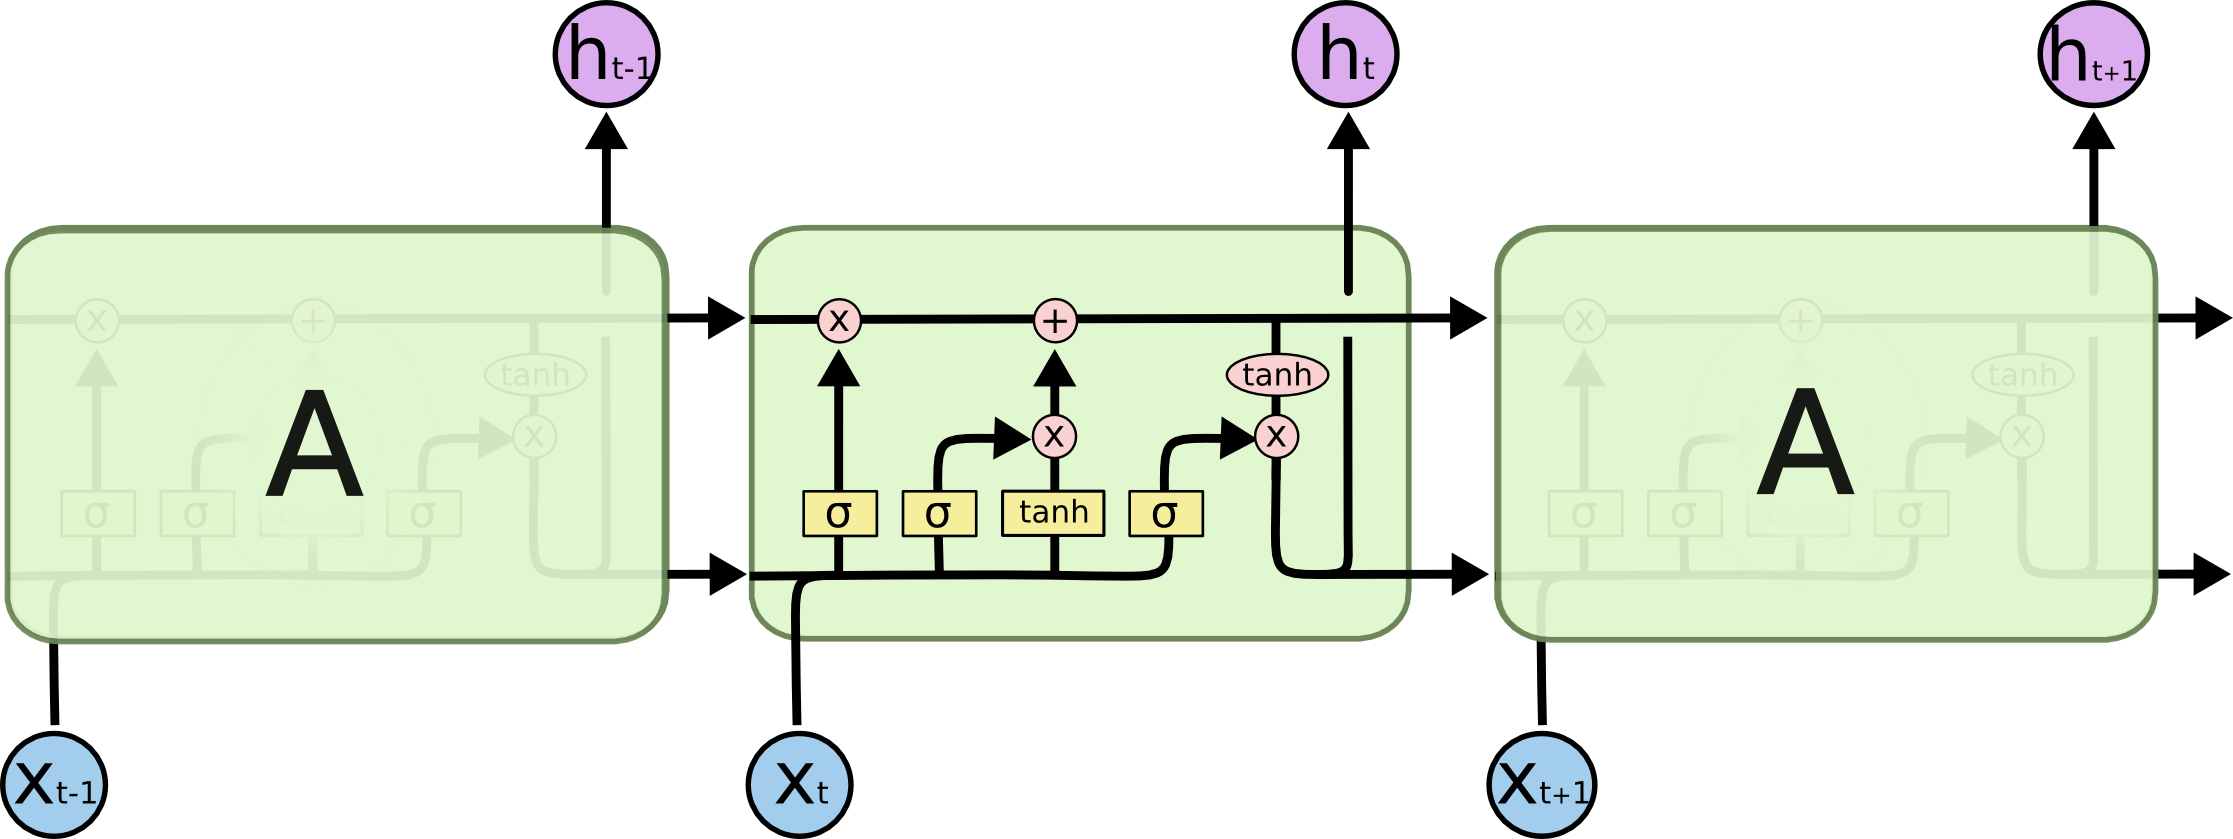
\includegraphics{Figures_LLM/lstm.png}

}

\caption{\label{fig-lstm}Long Short-Term Memory Network}

\end{figure}

In an LSTM network, there are three gates that are needed to pass
through. First is the gate that chooses which information to forget,
then the second gate decides which information to store. In the second
gate, we have two functions which decides which values will be updated
and what values will be used to update. Lastly, the third gate will
decide which information will be the output.

\emph{Drawback of RRN and LSTM} Now, while both networks are successful
in predicting the next word given a series of words, one major drawback
of these two networks is that they require their input data to be
processed sequentially, that is in order to process the next word of
input \(x_i\), we need the result of the previous input \(x_{i-1}\).

The \emph{attention} mechanism addresses this issue by stacking the
input in a matrix such that they can all be processed at the same time.
According to the paper ``Attention is all you need'', the authors
defined the attention function as the following:

\texttt{An\ attention\ function\ can\ be\ described\ as\ mapping\ a\ query\ and\ a\ set\ of\ key-value\ pairs\ to\ an\ output,\ where\ the\ query,\ keys,\ values,\ and\ output\ are\ all\ vectors.\ The\ output\ is\ computed\ as\ a\ weighted\ sum\ \ of\ the\ values,\ where\ the\ weight\ assigned\ to\ each\ value\ is\ computed\ by\ a\ compatibility\ function\ of\ the\ query\ with\ the\ corresponding\ key.}

Now, the attention mechanism is used in a neural network architecture
called a \textbf{transformer}.

Here is how the transformer neural network works:

\begin{enumerate}
\def\labelenumi{\arabic{enumi}.}
\tightlist
\item
  Tokenization
\end{enumerate}

Tokenization is the process of converting words or any natural language
to tokens which are the ones processed by our computers. There are three
main approaches in tokenization which are the following:

\begin{itemize}
\tightlist
\item
  Word-based: Split a sentence on spaces where generally, punctuation
  marks are also split into different tokens.
\item
  Subword-based: Split words into subwords. Example would be ``o c ca
  sion''.
\item
  Character-based: Split sentence into individual characters.
\end{itemize}

For example, taking the sentence ``Once again Mr.~Costner has dragged
out a movie for far longer than necessary.''

Using the \texttt{fastai} module in Python, we can implement the
following types of tokenization. For the word-based tokenization, we use
the following block of following code:



\end{document}
